\documentclass{article}

\usepackage[margin=1in]{geometry}
\usepackage{mathtools}
\DeclarePairedDelimiter{\ceil}{\lceil}{\rceil}

\usepackage{listings}
\renewcommand{\tt}[1]{\texttt{#1}}
%\newcommand{\linux}[1]{\begin{lstlisting}[language=bash] #1 \end{lstlisting}}
\lstnewenvironment{linux}{\lstset{language=bash}}{}


\begin{document}
\begin{center}
\Large{MA/CSSE Homework 7}\\
Due 5/12
\end{center}
\vspace{.25in}
\noindent{\textbf{Directions}}\\
  \begin{itemize}
   \item \textbf{Each problem must be self-contained in a file}, named
     properly, and \textbf{must compile using the
      command} \texttt{mpicc filename.c}\\

  \item Turn in each \tt{.c} file to the dropbox. \textbf{Do not
      create a \tt{.zip} file}

  \item On this homework you may not use any of the standard default
    MPI collective operations. 
  \end{itemize}


\section*{Problems}

\noindent{\textbf{Level:}Easy}\\
\begin{enumerate}
\item Create a file called \tt{bucketsort.c} that implements the
  bucketsort algorithm discussed in class, and that is represented in
  figure 4.10 (page 120) of the book.  Basically, the algorithm has
  the following steps:
  \begin{enumerate}
  \item The root processor reads in the data to sort.  
  \item The root processor divides the initial list, $L$, into $p$
    sub-lists, where $p$ is the number of processors. Let's call the
    $i^{th}$ sublist $L_i$. Each $L_i$ is  of length approximately
    $n/p$.  The root processor distributes $L_i$ to processor $i$. 
  \item Processor $i$ divides $L_i$ into ``sub buckets'',
    $B_{i,j}$.
    
  \item Each processor $i$ sends all of its sub-buckets $B_{ij}$ to
    the corresponding processor, $j$. 

  \item Each processor uses quicksort to sort its bucket.
    
  \item Each processor sends its data back to the root node to be
    appended to the final master list. 
  \end{enumerate}

The file \tt{bucketsort\_start.c} provides a start for you, and the
file \tt{bucketsort\_helpers.h} provides some utilities for parsing
the command line, printing usage, etc.  Note that \tt{quicksort} is
provided for you. 

You may compile the standard code using:\\
\tt{\$ mpicc -lm objs/bucketsort\_standard.<arch>.o -o
  bucketsort\_standard}
Notice that you need to link the math library using \tt{-lm}.

Here are the criteria to keep in mind:
\begin{enumerate}
\item You must produce the correct results.  Respect the \tt{--print}
  option, it is stored in the \tt{print\_things} field of the options
  struct. If the list is to be printed, print both the sorted and
  unsorted list out in the
  exact same format as the standard code. You must also respect the
  \tt{--produce\_outputfile} flag. 

\item Only the root processor should ever have a full copy of the
  list.  So, only it should read the input file if one is provided,
  and only root 0 should generate the random data if there is no input
  file provided. 
\item You must produce a file containing the sorted list -- this is
  taken care of with \tt{write\_outputfile}

\item You must use \tt{MPI\_Scatterv} to do the initial distribution
  of data from the root,  \tt{MPI\_Gatherv} to do the final collecting
  of data back to the master, and
  \tt{MPI\_Alltoallv} for the swapping of ``sub-buckets''.  Besides
  those communications, your other messages may total no more than
  $10p$ integers. 

\item Your code will be run with $1,2,4,8,16,$ and $32$ processes.
  Your code may take no more than $2$ times as long as the standard
  code in each case.  As with homework 6, you may skip some of this
  testing using the \tt{--max-proc=<n>} option to the
  \tt{test\_bucketsort.py} program. 

\end{enumerate}




\end{enumerate}

\newpage

\noindent{\textbf{Level:} Difficult}

Complete the problem above.  In addition:

\begin{enumerate}
\item \textit{Cellular Automaton} are a classic construct widely used
  in mathematics in computer science.  The have been used for strictly to model complex phenomena like traffic flow, spread of
  forest fire, population dynamics, and crime incidents in urban areas. The most famous
  cellular automaton was developed by John H. Conway in the 1960's,
  and is called the \textit{Game of Life}.
  Canway developed the game to illustrate that complex behavior can arise out of
  simple systems using only simple rules.  

  Cellular automata consist of an initial grid of cells, each cell may
  be in one of finitely many states.  The initial set of states is
  called the \textit{initial condition} of the cellula automata.  From
  the initial condition, the system progresses, from one
  \textit{generation} to another, following a prescribed set of rules. 

  In the Game of Life, we imagine that an organism may occupy each
  cell.  Therefore each cell has only two possible states, empty or
  occupied.  Each cell has eight neighboring cells.  The rules to
  transition from one generation to another are:
  \begin{itemize}
  \item Any organism with two or three neighboring organisms survives
    for another generation.
  \item Every organism with four or more neighbors dies from
    overpopulation.
  \item Every organism with one neighbor or none dies from isolation.
  \item Each empty cell adjacent to exactly three occupied neighbors
    will give birth to an organism. 
  \end{itemize}

  We assume that the board ``wraps around''. 

  For example, imagine that this were the initial state of a GOL
  board:

  \begin{center}
    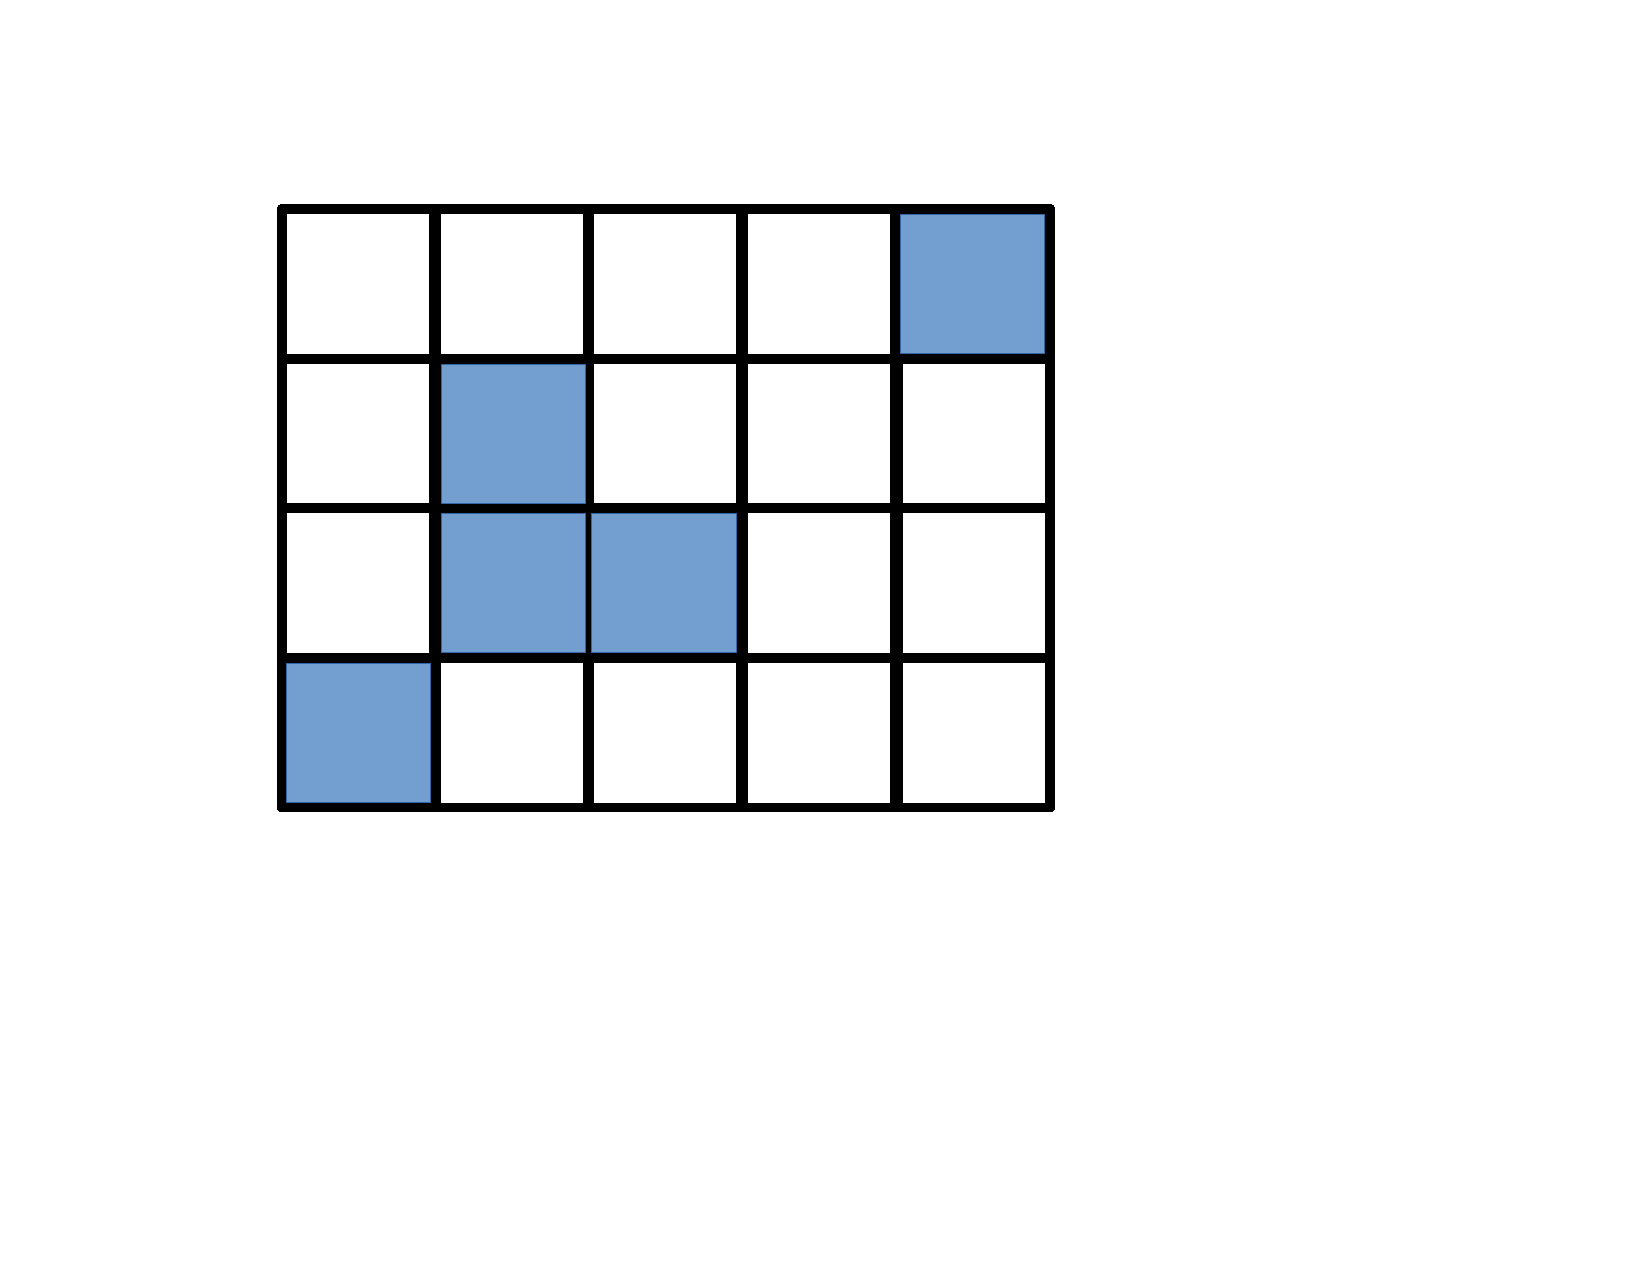
\includegraphics[trim={4cm 7cm 10cm 3cm},clip,width=4in]{figs/gol_0.pdf}
  \end{center}
  Following the rules above, the next generation of the board is:
  \begin{center}
    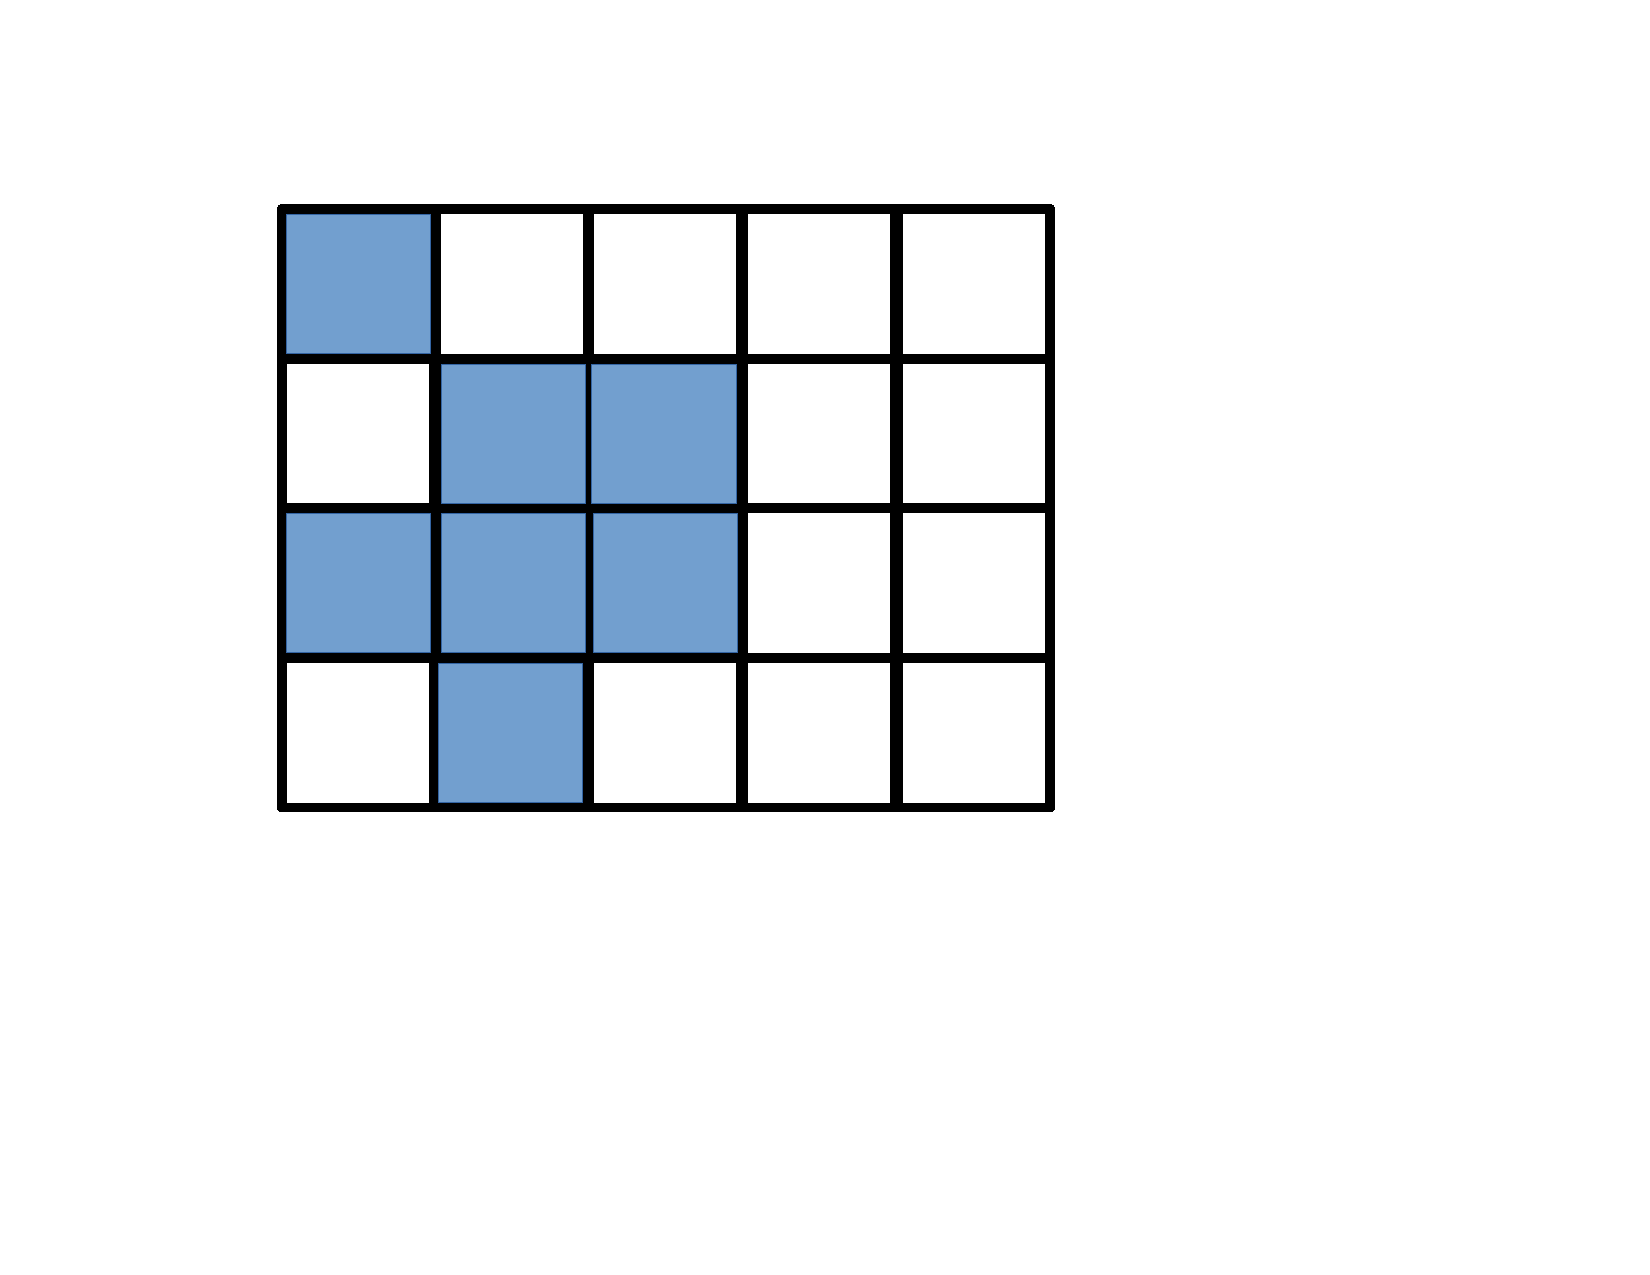
\includegraphics[trim={4cm 7cm 10cm 3cm},clip,width=4in]{figs/gol_1.pdf}
  \end{center}

In the file \tt{gol.c} write a program to play the game of life
using many processors.  The code in \tt{gol\_start.c},
\tt{gol\_helpers.h}, \tt{gol\_comm\_helpers.h} provide the code to
read and set the appropriate simulation options, utilities for
producing the output gif, and tools for use during the simulation. 

Suppose the grid is $m$ rows by $n$ columns, and that we have $p$
processors to use.  In the figure above, $m=4$, $n=5$.  Imagine
overlaying the grid with a \textit{block grid} of dimensions $M \times
N$, and assigning each processor to update only the cells that lie
within its assigned block.  In the figure below, $M=2$, $N=2$. 
\begin{center}
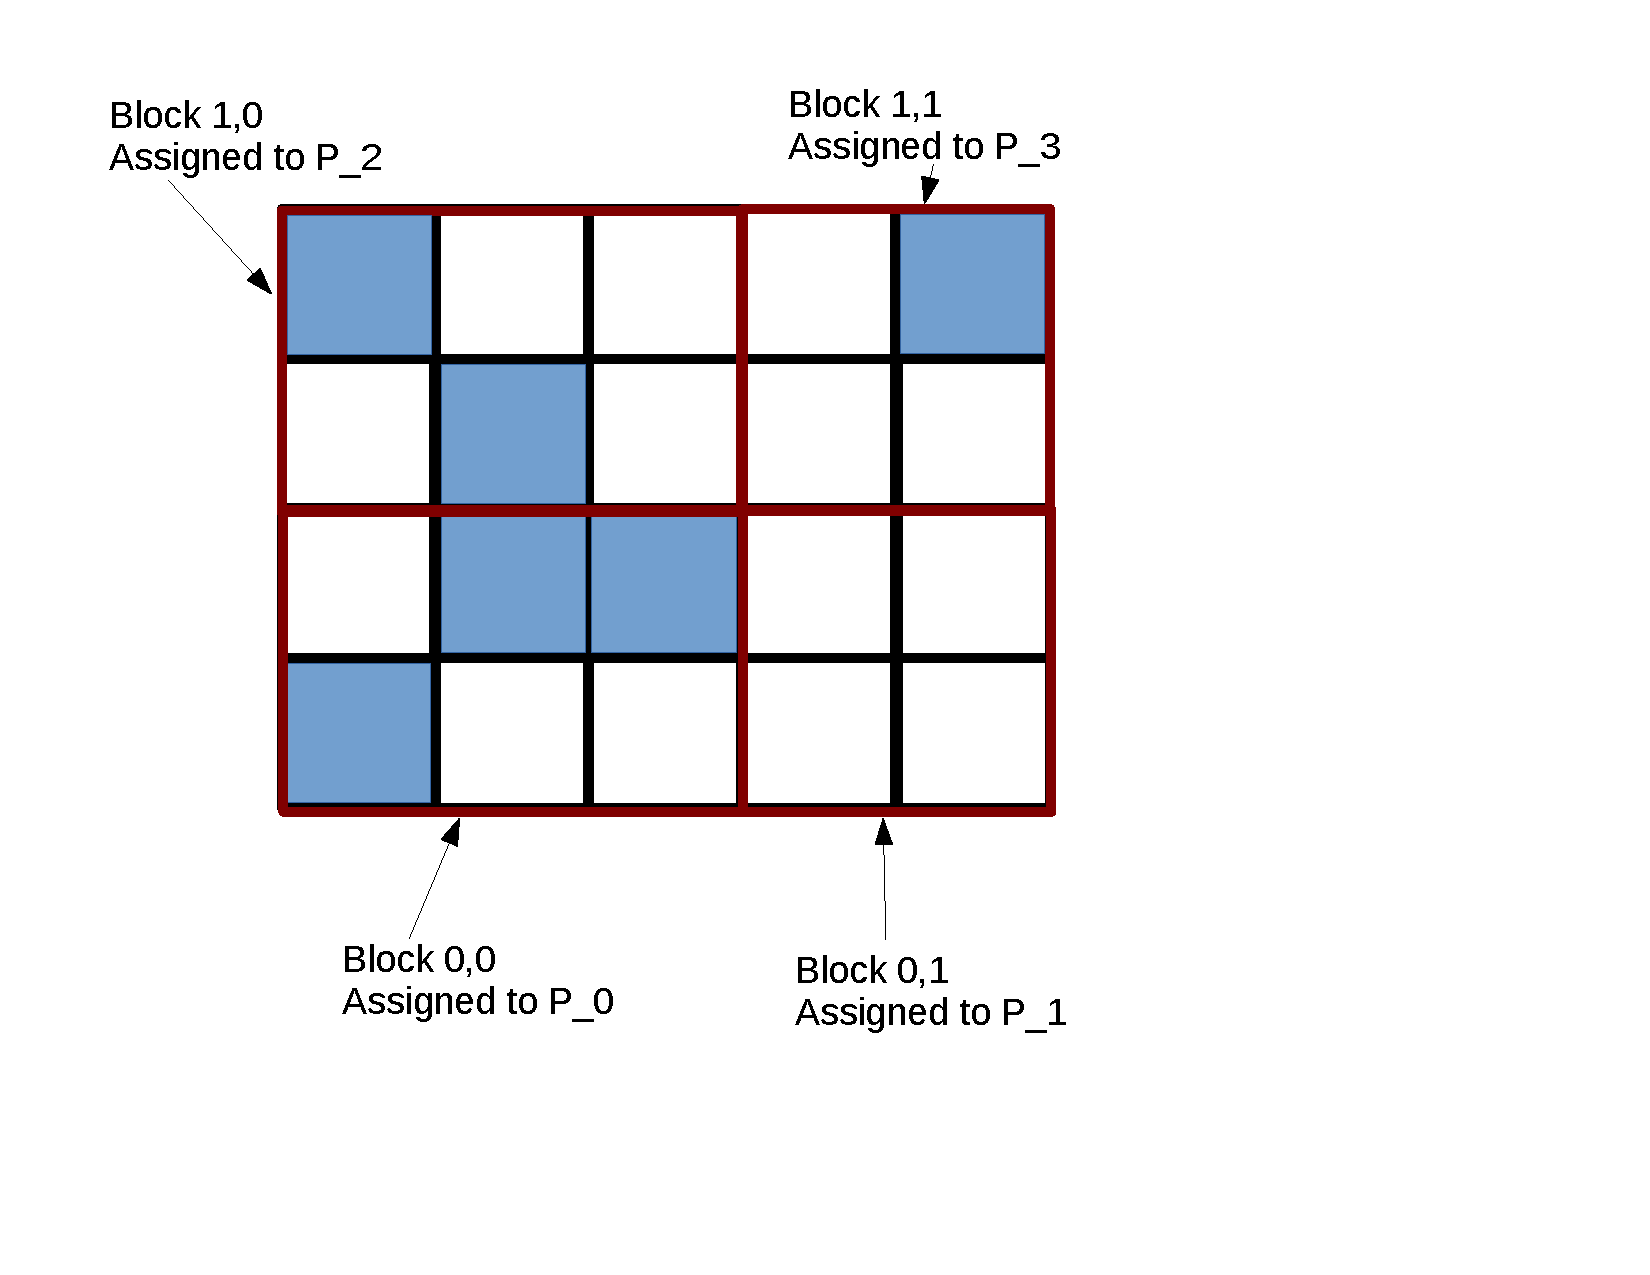
\includegraphics[trim={1.5cm 3.5cm 8cm 1.5cm},clip,width=5in]{figs/gol_1_block.pdf}
\end{center}

We can see that in order to update the cells in its block from
generation $t$ to $t+1$, each processor must receive information about
the cells on its border from its neighboring processors.  Similarly it
must sent the state the cells on its border to all neighboring
processors so that they may update their generation.  

Here are the facts you need to know about the simulation:
\begin{itemize}
\item The number of generations in \tt{options} includes the initial
  generation that is read in from file. 
\item The board wraps around in all directions, there is a function
  \tt{get\_state} in \tt{gol\_helpers} that will get the state of a
  board at generation $t$, row $i$, column $j$.  It handles wraparound
  properly, so that asking for row 1, column -1 will get the
  \textit{rightmost} entry of row 1.

\item The state of a cell $i,j$ at time $t$ can be set using
  \tt{set\_state}.  You \textbf{must} use \tt{set\_state} to set the
  state of the board every time -- it is how I keep track of how much
  work each processor does.  

\item All indexing is 0 based. 

\item Determining the dimensions of the block grid, and assigning
  blocks to processors is done for you.
  \begin{itemize}
  \item   In \tt{gol\_comm\_helpers.h}
  the function \tt{get\_block\_dims} returns the block dimensions $M$
  and $N$ to use on a board with dimensions $m$ and $n$ when using
  $n_{procs}$ processors. 

\item \tt{get\_block\_coords} returns the coordinates (block row,
  block column) of the block assigned to processor \tt{rank} if the
  block grid is $M \times N$.

\item \tt{block\_coords\_to\_rank} returns the rank of the processor
  assigned to block $b_i, b_j$ (block row, block column) if the block
  grid is $M \times N$.  This handles wraparound correctly, so asking
  for the processor assigned to $-1,0$ returns the processor assigned
  to $4,0$ if the block grid has 5 rows.   

\item \tt{get\_assignment} returns the leftmost column, rightmost
  column, bottommost row and topmost row (all inclusive), that the
  processor with block indices $b_i,b_j$ should work on if the board
  is $m\times n$ and the block grid is $M\times N$. 
  \end{itemize}

\item At each generation, each processor must share only the correct
  amount of data (the number of cells on its perimeter) with its
  neighboring processes.  Each processor should send its boundary data
  to itself, if it is its own neighbor (simplifies the coding a lot). 

\item In order to reduce the potential for deadlock, you must use the
  \tt{MPI\_Sendrecv} command to transfer all boundary data. 

\item At the end of the simulation, every processor must send its
  complete information back to the root processor.  The root processor
  must then produce an animated gif of the game. 
  \begin{itemize}
  \item The function \tt{copy\_board\_range\_to\_buffer} copies a
    specified section of the board into a contiguous buffer suitable
    for sending, it handles wrapping around properly. 

  \item The function \tt{copy\_buffer\_to\_board\_range} copies a
    buffer to a specified chunk of the board, it also handles
    wrap-around correctly.  
  \end{itemize}

\item The files \tt{gol\_serial.c} and \tt{gol\_serial\_helpers.h}
  give you a complete serial implementation of the game.  The files
  \tt{gol\_start.c} gives you a start on the parallel version, and
  \tt{gol\_helpers.h} and \tt{gol\_comm\_helpers.h} are the
  appropriate helper functions. 

\item It is perfectly reasonable on this assignment to modify my
  helper files, or to create your own helper files.  So, you
  \textbf{must submit all files required to compile your code,
    including the ones I distribute to you}.  Your code must compile
  with a simple\\
\tt{mpicc gol.c}
Feel free to modify any of my functions that you want, with the
exception of \tt{set\_state}. You do not need to submit any of the
initial condition files, etc. 

\item Your code will be run with $1,2,4,8,16,$ and $32$ processes.
  Your code may take no more than $2$ times as long as the standard
  code in each case.  As with homework 6, you may skip some of this
  testing using the \tt{--max-proc=<n>} option to the
  \tt{test\_gol.py} program. 

\item You may use \tt{rang\_gol\_board.c} to create random initial
  states if you like. 

\end{itemize}


\end{enumerate}



\end{document}
